\documentclass{article}
\usepackage{graphicx}
\title{HISTORICAL CONTEXT OF FIVE (5) PROGRAMMING LANGUAGES}
\author{Arinzechi Adaobi Favour}
\begin{document}
	\section{MAPLE}
	
	\textbf{FOUDER}:  Waterloo Maple (Maple soft)

	\textbf{\underline{History of maple (programming language)
	}}
     Maple official release date was in 1982. It was developed by Waterloo Maple ( Maple soft ). It came about when researchers at university of waterloo  wanted to buy a powerful computer strong enough to take on the lisp-based computer algebra system macsyma.  so instead they developed maple  which  would run on low cost computers and  could also be portable. These researchers began writing maple from  BCPL . It was first released in 1982.  Then over time Maple had an exponential growth.  Maple is technical developed to cover areas such as data processing.
     
     \underline{Advantage  of maple}
       
       It provides an intellectual environment In solving technical problems due to the fact that it can carry out symbolic, numeric and graphical computations. It is a very powerful language even though it was written in C, Java , Maple.
       
       But no one uses maple again because it is slow, instead people use mathematica.
       
       Maple is more or less a mathematical software
       
       \underline{Examples of applications
       }
       
       Fractal leaf generator, Knight’s Tour, The SEIR model with births and deaths. Etc.
       
       Maple IDE- comes with features like
       Powerful Maple code editor, automatic indenting, source code validation which makes it easy to use.
       
       \textbf{IDE} ( Integrated Development Environment) just enables programmers to incorporate the different aspects of writing a computer  program.
       
       Related programs – C , Java
       
     \newpage  
     
\begin{figure}
	\centering
	\includegraphics[width=\linewidth]{"Maple-3-BIG (1).jpg"}
	\caption{image of maple}
	\label{fig:maple-3-big-1}
\end{figure}

  \newpage
  \section{ HTML ( Hypertext Markup Language)}
 
 
\begin{itemize}
	\item\underline{Founder:}  sir Tim Berners- Lee in late 1991 but official released in 1995 as HTML 2.0
	
	\item The first version of HTML (HTML 1.0) was released in1993 to enable data sharing, which would be very accessible  .
	
	\item Then came HTML 2.0 , HTML 3.0, HTML 4.01 and HTML 5.0, which was released in 2012 is still used till date.
	\item For  example 
	<!DOCTYPE html> - illustrates that the document is html
	
	<p>-paragraph
	
	<h1>- large heading
	
	<body>- document itself
	
	<title>- the title
	
	<head>-contains information about the page
	
	<br>- an empty element	
	\item IDE – intellij idea is good for CSS IDE but also supports HTML and simple text editor which allows you to write codes
	
	\item The HTML 5.0 is a really good version because works with almost all IDE’s very easily
	\end{itemize}
	\newpage
	
	\section{FORTRAN}
\textbf{\underline{Developer :}}	  John Backus

It was developed by a team of programmers at IBM led by John Backus(Dec. 3 , 1924 –March 17,2007) in 1957. It is called FORTRAN ( Formula Translation)  because of how it is developed to enable easy translation of math formulas into code. John Backus made a proposal to his colleagues .When it was first released people were skeptical about it, eventually it quickly gained acceptance  . It was the first high-level language using compiler. It is now one of the oldest programming languages . it was developed with the intention of making a programming language which was simple to learn.

IT made coding so much easy , programmers were able to focus more on execution than the process of debugging the code. FORTRAN also develop several dialects ( due to some modification of some programmers for their best interest. The ASS reviewed the problem then produced a version FORTRAN’66 then there was FORTRAN’77(1978) and the latest which is still in use till date FORTRAN’90(1991). It was a huge success since in the past programs were written in machine language or assembly language, which required the programmers to write instructions in binary or hexadecimal. Fortran is used for factory automation control, storm drainage design.

	\begin{itemize}
		\item Fortran  similar programs- C, C sharp, F sharp.
		\item IDE used Fortran – Eclipse- Photran , visual studio, simply Fortran, Plato. Etc.
		\end{itemize}
	
		\begin{figure}
			\centering
			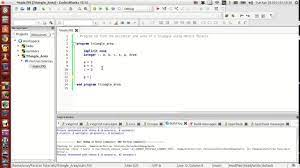
\includegraphics[width=0.7\linewidth]{fortan}
			\caption{image of fortran}
			\label{fig:fortan}
		\end{figure}
	
	\section{RUBY}
	\textbf{\underline{FOUNDER:}}Yukihiro Matsumoto
	
		\underline{HISTORY}
		
		\begin{itemize}
			\item Ruby was developed in the mid 1990s but made its first appearance in 1995. It is an interpreted high-level language. Yukihiro wanted an object-oriented scripting language that he liked and was not to complex ,he had tried Perl and Python and did not like it so he decided to make his own.
			\item The name Ruby was proposed before any code had been written for the project. It was the birthstone of one of his colleagues. By 2000 Ruby was more popular than Python in Japan. Yukihiro’s initial aim of Ruby was just to design a good a language that he enjoyed and others can enjoy and reducing the programming work. Ruby is primarily for building web applications , but Python is easier to learn because it is explicit and faster.
			
			\item  Features of Ruby:Vital reflect ion ,default argument etc.
			Similar programming language: Perl and Python.
			
			
		\end{itemize}
	\begin{figure}
		\centering
		\includegraphics[width=0.7\linewidth]{../../Downloads/RUBY.J}
		\caption{IMAGE OF RUBY}
		\label{fig:ruby}
	\end{figure}
\section{BASIC (BEGINNERS ALL PURPOSE SYMBOLIC INSTRUCTION CODE)}
\textbf{\underline{FOUNDER:}}
	John G. Kemeny, Thomas E. KurtZ
	
	\textbf{HISTORY}
	
	\begin{itemize}
		\item John  G. Kemeny and Thomas E. Kurtz released the original version in May 1st 1964. BASIC is a high-level programming language. They developed this less complex programming language which enables students in fields of science and mathematics to work with the use of computers. They also developed Dartmouth Time Sharing System (DTSS) which allowed users to modify and run BASIC schemes at the same time. Basic is mostly used for business applications .They initial tried to develop programs like DOPE ( Dartmouth Oversimplified Programming experiment) and DARSIMCO (Dartmouth simplified code ) but they weren’t too successful. The project was gifted a $300,000 grant  from the National Science Foundation which they were able to use to purchase GE-225 process control computer.
		
		\item IDE for BASIC (Beginners)- visual Studio, Webstorm etc.
		
		\item Related programming language – 83pure Basic , Java, python.
		
	\end{itemize}
	\begin{figure}
		\centering
		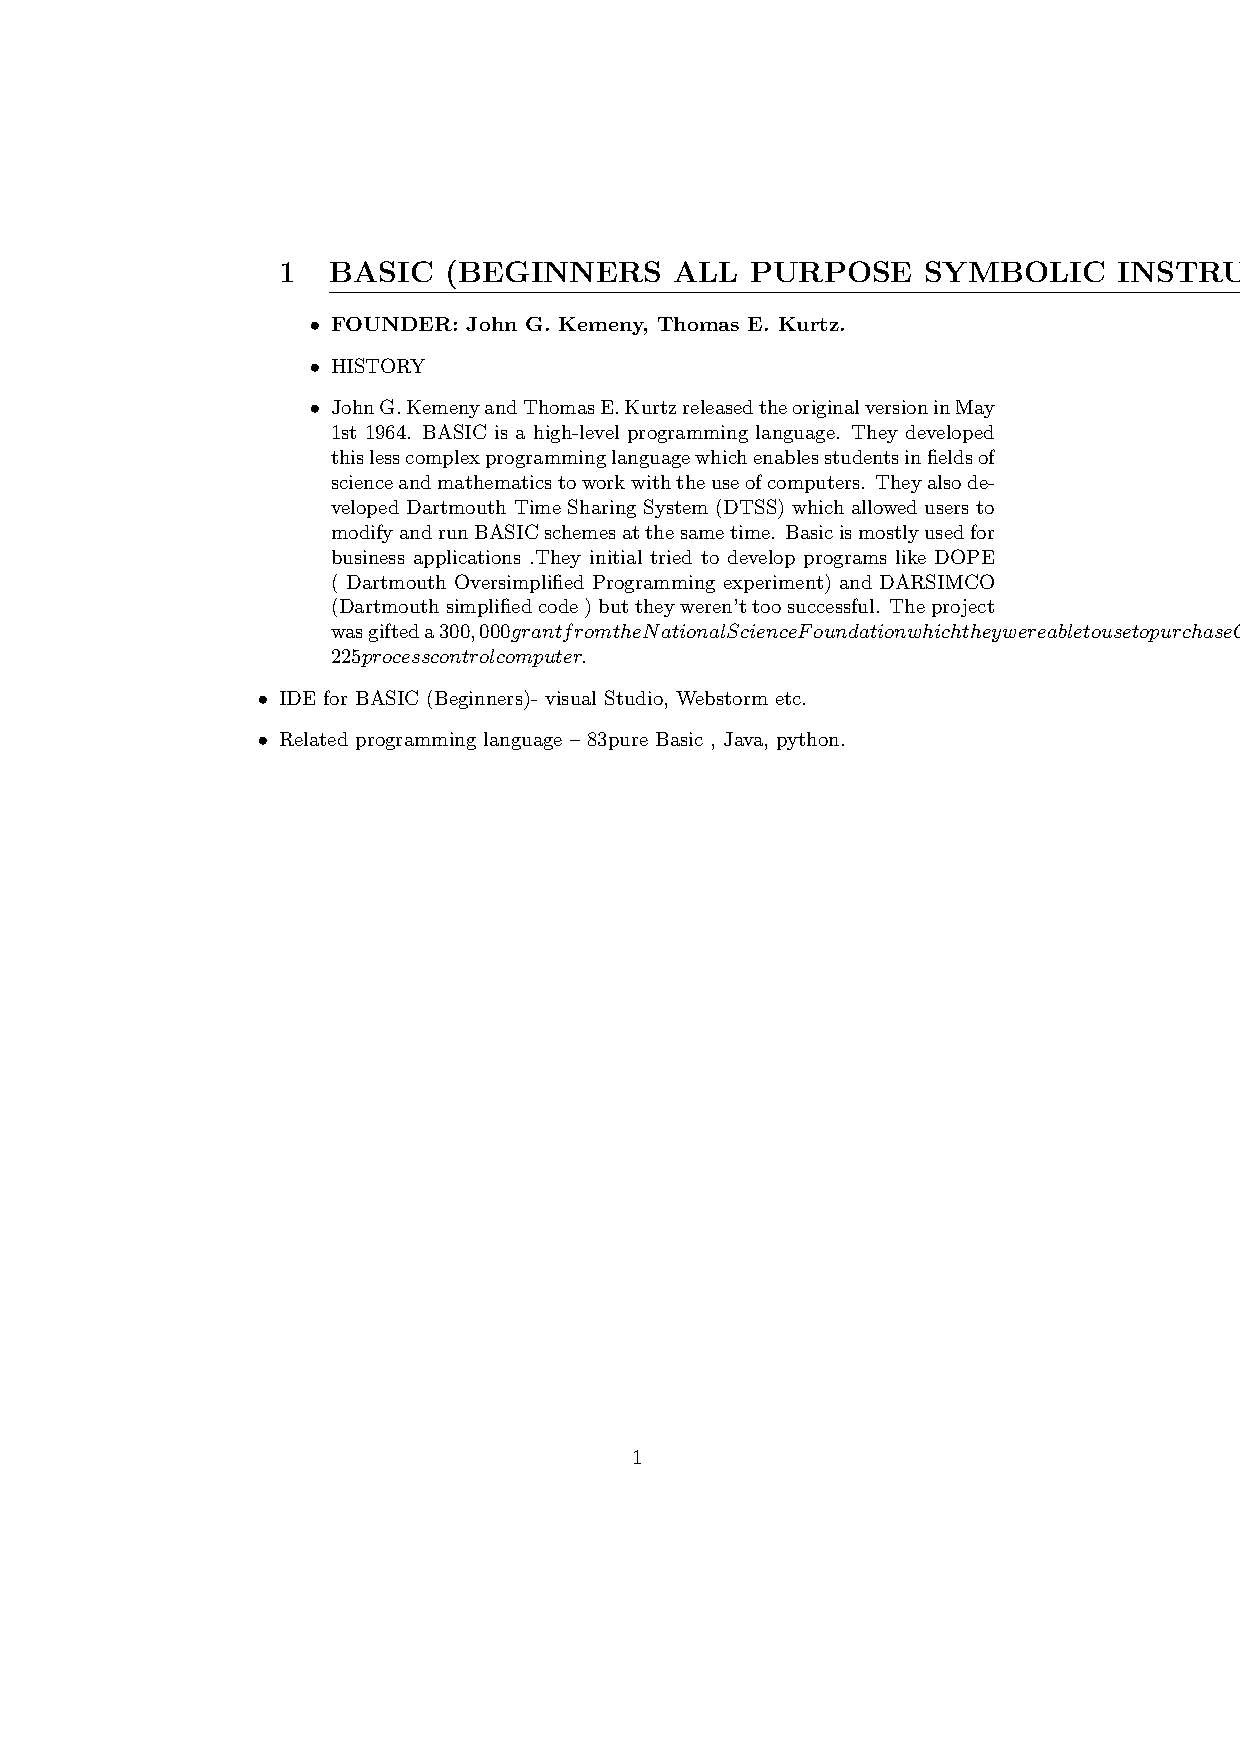
\includegraphics[width=0.7\linewidth]{../../Downloads/basic}
		\caption{IMAGE OF BASIC}
		\label{fig:basic}
	\end{figure}
	
	
	
	

     
 
\end{document}

	
	
